\chapter{Grupos de Homotopía}
\section{Grupos de homotopía de mayor orden}
El grupo fundamental $\homot{1}{X, x_0}$ ya es conocido. Además, anteriormente ya hemos definido los grupos de homotopía de un espacio:
\[ \homot{n}{X, x_0} = [(I^n, \partial I^n), (X, x_0)], \text{ donde } I^n = [0,1]^n \]
Definimos, dadas $f,g : (I^n, \partial I^n) \longrightarrow (X, x_0)$,
\[
(f + g)(s_1, \ldots, s_n) = 
\begin{cases}
f(2s_1, s_2, \ldots, s_n) & \text{si } s_1 \leq \frac{1}{2} \\
g(2s_1 - 1, s_2, \ldots, s_n) & \text{si } s_1 \geq \frac{1}{2}
\end{cases}
\]
Esta operación induce en las clases de homotopía una operación que es asociativa:
\[
(f + g) + h \simeq f + (g + h) \qquad (\text{relativa a } \partial I^n)
\]
admite elemento neutro:
\[
f + c_{x_0} \simeq f \simeq c_{x_0} + f \qquad (\text{relativa a } \partial I^n)
\]
y elemento inverso:
\[
f^{-1} (s_1, \ldots, s_n) = f(1 - s_1, \ldots, s_n) \qquad (\text{relativa a } \partial I^n)
\]
Se podría pensar sobre otras posibles operaciones cambiando la coordenada elegida. Podemos definir las operaciones
\[
(f +_i g)(s_1, \ldots, s_n) = 
\begin{cases}
f(s_1, \ldots, 2s_i, \ldots, s_n) & \text{si } s_i \leq \frac{1}{2} \\
g(s_1, \ldots, 2s_i -1, \ldots, s_n) & \text{si } s_i \geq \frac{1}{2} \\
\end{cases}
\]
Pero resulta que estas operaciones coinciden. Esto puede verse haciendo uso del siguiente resultado:
\begin{prop}[(Argumento de Eckmann-Hilton)]
Sea $X$ un conjunto dotado de dos operaciones $\bullet$ y $\circ$ y supongamos que 
\begin{enumerate}
\item $\bullet$ y $\circ$ poseen la misma unidad.
\item $\forall a,b,c,d$ se verifica que
\[
(a \bullet b) \circ (c \bullet d) = (a \circ c) \bullet (b \circ d) 
\]
\end{enumerate}
Entonces $\bullet$ y $\circ$ coinciden y son asociativas y conmutativas.
\end{prop}
\begin{demo}
Sean $a,b \in X$ y sea $1$ la unidad de ambas operaciones. Entonces
\begin{align*}
a \circ b &= (1 \bullet a) \circ (b \bullet 1) = (1 \circ b) \bullet (a \circ 1) = b \bullet a  \\
&= (b \circ 1) \bullet (1 \circ a) = (b \bullet 1) \circ (1 \bullet a) = b \circ a
\end{align*}
Esto demuestra la igualdad de las operaciones y la conmutatividad. Veamos la asociatividad:
\[
(a \bullet b) \bullet c = (a \bullet b) \bullet (1 \bullet c) = (a \bullet 1) \bullet (b \bullet c) = a \bullet (b \bullet c)
\]
\end{demo}
Por tanto, como estas operaciones verifican las condiciones de la proposición, obtenemos el siguiente resultado inmediatamente:
\begin{teor}
Si $n \geq 2$, entonces $\homot{n}{X, x_0}$ es abeliano.
\end{teor}
El caso $n=1$ no puede contemplarse ya que al trabajar únicamente con una coordenada no disponemos de otra operación distinta con la que aplicar el Argumento de Eckmann-Hilton.
\begin{custom}[Observaciones]
\begin{enumerate}
\item En el caso que tengamos $C$ componente arcoconexa que contiene a $x_0$, entonces $\homot{n}{X, x_0} = \homot{n}{C, x_0}$. Por lo tanto, supondremos $X$ arcoconexo.

\item Las aplicaciones $ (I^n, \partial I^n) \longrightarrow (X, x_0)$ coinciden con las aplicaciones definidas en el cociente $(\faktor{I^n}{\partial I^n}, \ast) \longrightarrow (X, x_0)$. Pero $S^n = \faktor{I^n}{\partial I^n}$ y con estas identificaciones, la estructura de grupo es la que conocíamos \par
\begin{figure}[h]
\centering
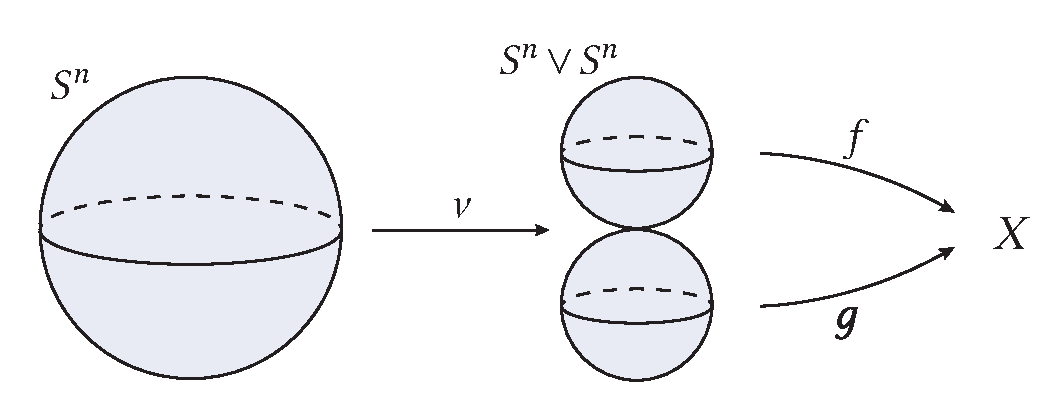
\includegraphics[width = 0.5\textwidth]{images/ejgruphomot}
\end{figure}
\[S^n \longrightarrow S^n \vee S^n \stackrel{f \vee g}{\longrightarrow} X \]
\end{enumerate}
\end{custom}
Veamos ahora que si cambiamos el punto base obtenemos grupos de homotopía isomorfos (al igual que ocurría para $\pi_1$). \par
Tomamos dos puntos $x_0, \ x_1 \in X$ y un camino $\gamma : I \longrightarrow X$ tal que $\gamma(0) = x_0$, $\gamma(1) = x_1$. A cada aplicación $f : (S^n, p_o) \longrightarrow (X, x_0)$ le asociamos una aplicación
\[
\gamma_f : (S^n, p_0) \longrightarrow (X, x_0)
\]
definida de la siguiente forma: \par
Encogemos el dominio de f a un cubo menor concéntrico en $I^n$, e insertamos el camino $\gamma$ en cada segmento radial entre este cubo y $\partial I^n$. \nts{Insertar imagen p64, explicar $I^n$} \par
Se tienen entonces las siguientes propiedades: \par
\begin{enumerate}
\item $\gamma_{(f+g)} \simeq \gamma_f + \gamma_g$
\item $(\gamma \eta)_f \simeq \gamma_{\eta_f}$
\item ${c_{x_1}}_f \simeq f$
\end{enumerate}
Entonces, para cada $\gamma$ definimos
\begin{align*}
\beta_\gamma : \homot{n}{X, x_1} &\longrightarrow \homot{n}{X, x_0} \\
[f] &\longmapsto [\gamma_f]
\end{align*}
que es un morfismo de grupos, cuyo inverso es $\beta_{\gamma^{-1}}$. Por tanto:
\begin{teor}
Dados $x_0, x_1 \in X$, se tiene que $\homot{n}{X, x_1} \cong \homot{n}{X, x_0}$ mediante $\beta_\gamma$.
Es más, si $n=1$,
\begin{align*}
\homot{1}{X, x_1} &\stackrel{\cong}{\longrightarrow} \homot{1}{X, x_0} \\
[\alpha] &\longmapsto [\gamma \alpha \gamma^{-1}]
\end{align*}
\end{teor}
De las propiedades también se obtiene
\begin{teor}
La aplicación 
\begin{align*}
\homot{1}{X, x_0} \times \homot{n}{X, x_0} &\longrightarrow \homot{n}{X, x_0} \\
[\gamma], [f] &\longmapsto [\gamma_f]
\end{align*}
es una acción.
\end{teor}
Cuando $n = 1$, la acción es por conjugación, y hace al grupo abeliano $\homot{n}{X, x_0}$ un $\bb{Z}[\homot{1}{X}]$-módulo mediante
\[
\left( \sum_i n_i \gamma_i \right) \alpha = \sum_i n_i {\gamma_i}_\alpha
\]
Decimos que el espacio es abeliano si la acción de $\homot{1}{X, x_0}$ en $\homot{n}{X, x_0}$ es trivial. En particular, si $n=1$, esta condición nos dice que $\homot{1}{X, x_0}$ es abeliano. \par
Si tenemos $f : (X, x_0) \longrightarrow (Y, y_0)$ aplicación continua, podemos definir
\begin{align*}
\homot{n}{f} : \homot{n}{X, x_0} &\longrightarrow \homot{n}{Y, y_0} \\
[\alpha] & \longmapsto [f \circ \alpha]
\end{align*}
Con esta definición, tenemos:
\begin{prop}
$\pi_n$ es un funtor en la categoría homotópica con valores en la categoría de los grupos:
\begin{enumerate}
\item $\homot{n}{f}(a+b) = \homot{n}{f}(a) + \homot{n}{f}(b)$
\item $\homot{n}{Id} = Id_{\homot{n}{X}}$
\item Si $f \simeq g$, entonces $\homot{n}{f} = \homot{n}{g}$.
\end{enumerate}
\end{prop}
Por tanto, si $f : (X, x_0) \longrightarrow (Y, y_0)$ es una equivalencia de homotopía, entonces $\homot{n}{f}$ es un isomorfismo. En efecto, existe $g$ tal que $f \circ g \simeq Id_{(Y, y_0)}$ y $g \circ f \simeq Id_{(X, x_0)}$. Tenemos que $\homot{n}{f \circ g} = \homot{n}{f} \circ \homot{n}{g}$ ya que:
\[
\homot{n}{f \circ g}([\alpha]) = [f \circ g \circ \alpha] = \homot{n}{f}([g \circ \alpha]) = \homot{n}{f} \circ \homot{n}{g}([\alpha])
\]
Luego tenemos que 
\begin{align*}
\homot{n}{f \circ g} = \homot{n}{f} \circ \homot{n}{g} = Id \\
\homot{n}{g \circ f} = \homot{n}{g} \circ \homot{n}{f} = Id
\end{align*}
Y así, $\homot{n}{f}$ es un isomorfismo.
\section{Grupos de homotopía relativa}
Vamos a generalizar los grupos de homotopía. Para ello construiremos los llamados grupos de homotopía relativa. Para ello tomamos $x_0 \in A \subset X$ y consideramos $I^{n-1} \subset I^n$ como los puntos con última coordenada $0$ \nts{Añadir imagen p68}
y tomamos $J^{n-1} = \partial I^n - I^{n-1}$. \par
Se define entonces el grupo de homotopía relativa $n$-ésimo como
\[
\homot{n}{X, A, x_0} = [(I^n, \partial I^n, J^{n-1}), (X, A, x_0)]
\]
Se verifica que $\homot{n}{X, x_0} = \homot{n}{X, x_0, x_0}$. \par
Con la anterior operación definida, $\homot{n}{X, A, x_0}$ es un grupo si $n \geq 2$ y es abeliano si $n \geq 3$. \par
En el caso $n = 1$, tenemos que $\partial I = \{0,1\}$, $I^{n-1} = I^0 = \{0\}$, $J^0 = \{0\}$. Por tanto
\[
\homot{1}{X, A, x_0} = \text{clases de homotopía relativa a } x_0 \text{ de caminos qur van a } A \text{ en } x_0.
\]
que no es un grupo. \par
También podemos ver $\homot{n}{X, A, x_0}$ como $[(D^n, S^{n-1}, p_0), (X, A, x_0)]$, ya que colapsando $J^{n-1}$ a un punto, transforma $(I^n, \partial I^n, J^{n-1})$ en $(D^n, S^{n-1}, p_0)$ y le damos la estructura de grupo \nts{Insertar imagen p70} \par
Tenemos entonces el siguiente resultado:
\begin{teor}
La aplicación $ f : (D^n, S^{n-1}, p_0) \longrightarrow (X, A, x_0)$ representa el elemento neutro de $\homot{n}{X, A, x_0}$ si y sólo si $f \simeq g$ relativa a $S^{n-1}$ para algún $g$ con $Im\ g \subset A$.
\end{teor}
\begin{demo}
Supongamos que $f \simeq g$ relativo a $S^{n-1}$ e $Im \ g \subset A$. Entonces existe $H : (D^n, S^{n-1}, p_0) \longrightarrow (X, A, x_0)$. Por tanto, $[f] = [g]$ en $\homot{n}{X, A, x_0}$. Si tomamos $F: (D^n, p_0) \times I \longrightarrow (D^n, p_0)$ un retracto de deformación de $D^n$ en $p_0$, entonces 
\begin{align*}
g \circ F : D^n \times I \longrightarrow X \\
g \circ F (p,0) = g(p) \in A \\
g \circ F (p,1) = g(p_0) = x_0 \\
g \circ F (p_0, t) = x_0 \ \forall t \in I \\
\end{align*}
Luego $g \simeq 0$ y así $[f]=[g]=0$. \par
Recíprocamente, supongamos que $[f]=0$. Entonces existe $H: (D^n, S^{n-1}, p_0) \times I \longrightarrow (X, A, x_0) $. Si restringimos $H$ a una familia de discos $D^n \times I$ empezando por $D^n \times \{0\}$ y terminando por $D^n \times \{1\} \cup S^n \times I$, tenemos $F_t: H \vert_{D^n \times \{t\} \cup S^{n-1} \times [0, t]}$ \par
Todos los $n$-discos tienen el mismo borde $S^{n-1}$, luego $F : f \simeq g$ relativo a $S^{n-1}$ e $Im \ g \subset A$. \par
\nts{Mirar de nuevo, buscar en Spanier P372}
\end{demo}

Al igual que hicimos para los grupos de homotopía, dada una aplicación $\varphi :  (X, A, x_0) \longrightarrow (Y, B, y_0)$, esta induce un morfismo entre los grupos de homotopía relativa, $\homot{n}{\varphi} : \homot{n}{X, A, x_0} \longrightarrow \homot{n}{Y,B,y_0}$. Por tanto, considerando las inclusiones $i : (A, x_0) \longrightarrow (X, x_0)$ y $j: (X, x_0, x_0) \longrightarrow (X, A, x_0)$, éstas determinan morfismos
\begin{align*}
\homot{n}{i}&: \homot{n}{A, x_0} \longrightarrow \homot{n}{X, x_0} \\
\homot{n}{j}&: \homot{n}{X, x_0, x_0} \longrightarrow \homot{n}{X, A, x_0}
\end{align*}
Por otra parte, dada una aplicación $f: (D^n, S^{n-1}, p_0) \longrightarrow (X, A, x_0)$, la restricción $f \vert_{S^{n-1}} : (S^{n-1}, p_0) \longrightarrow (A, x_0)$ determina un morfismo $\partial : \homot{n}{X, A, x_0} \longrightarrow \homot{n-1}{A, x_0}$ llamado aplicación borde. \par
Entonces, tenemos el siguiente resultado:
\begin{teor}
La sucesión
\begin{align*} 
\ldots \longrightarrow \homot{n}{A, x_0} \stackrel{\homot{n}{i}}{\longrightarrow} \homot{n}{X, x_0} \stackrel{\homot{n}{j}}{\longrightarrow} \homot{n}{X, A, x_0} \stackrel{\partial}{\longrightarrow} \homot{n-1}{A, x_0} \longrightarrow \ldots \\
\ldots \longrightarrow \homot{1}{X, A, x_0} \longrightarrow \homot{0}{A, x_0} \homot{0}{X, x_0}
\end{align*}
es exacta.
\end{teor}
\begin{demo}
Veamos la exactitud en $\homot{n}{X, x_0}$. Consideremos la composición $\homot{n}{i} \circ \homot{n}{j} = \homot{n}{k}$. Veamos que es $0$. $k = i \circ j : (A, x_0, x_0) \longrightarrow (X, A, x_0)$. Consideremos ahora una función $f : (D^n, S^{n-1}, p_0) \longrightarrow (A, x_0, x_0)$. Así $k \circ f : (D^n, S^{n-1}, p_0) \longrightarrow (X, A, x_0)$ representa al neutro de $\homot{n}{X, A, x_0}$ por el teorema anterior. \par
Veamos ahora que $Ker \ \homot{n}{j} \subset Im \ \homot{n}{i}$. Sea $[f] \in Ker \ \homot{n}{j}$. Entonces $[f]$ representa al neutro en $\homot{n}{X, x_0}$. Por tanto, existirá $g$ tal que $f \simeq g$ relativa a $S^{n-1}$ con $Im \ g \subset A$. Así, $\homot{n}{i}[g] = [f] \in Im \ \homot{n}{i}$. \par
\nts{¿Completar con el resto de demost de exactitud?}
\end{demo}

\section{$n$-conexidad de un espacio}
\begin{defin}
Un espacio topológico $X$ con punto base $x_0$ se dice $n$-conexo si $\homot{i}{X, x_0} = 0$ para todo $i \leq n$.
\end{defin}
Con esta definición, que un espacio sea $0$-conexo quiere decir que es arcoconexo, y que sea $1$-conexo significa que el espacio es símplemente conexo. \par
Como $n$-conexidad implica $0$-conexidad, la mención del punto base de un espacio $n$-conexo no es importante. \par
Así, las siguientes condiciones son equivalentes:
\begin{enumerate}
\item $\homot{n}{X, x_0} = 0$ para todo $i \leq n$ y todo $x_0 \in A$
\item Cada aplicación $S^i \longrightarrow X$ es homotópicamente trivial para todo $i \leq n$.
\item Cada aplicación $S^i \longrightarrow X$ se extiende a $D^{n+1}$ para todo $i \leq n$.
\end{enumerate}
De la misma forma, para un par $(X, A)$ son equivalentes las siguientes condiciones:
\begin{enumerate}
\item Cada aplicación $(D^i, S^{i-1}) \longrightarrow (X, A)$ es homótopa relativa a $S^{n-1}$ a una aplicación $D^i \longrightarrow A$.
\item Cada aplicación $(D^i, S^{i-1}) \longrightarrow (X, A)$ es homótopa en $[(D^i, S^{i-1}), (X, A)]$ a una aplicación $D^i \longrightarrow A$.
\item Cada aplicación $(D^i, S^{i-1}) \longrightarrow (X, A)$ es homótopa en $[(D^i, S^{i-1}), (X, A)]$ a una constante $D^i \longrightarrow A$.
\item $\homot{n}{X, A, x_0} = 0$ $\forall x_0 \in A$.
\end{enumerate}
Para el caso $i = 0$, $\homot{0}{X, A, x_0}$ no está definido, por tanto, decimos que el par $(X, A)$ es $n$-conexo si se verifica una de las cuatro condiciones para $i > 0$ y si se verifica una de las tres primeras cuando $i=0$.

\section{Aplicaciones de la sucesión exacta de un par $(X,A)$}
Veamos ahora varios resultados que hacen uso de esta sucesión exacta.
\begin{teor}
Sea $p : E \longrightarrow B$ una fibración. Tomamos $b_0 \in B$ y un punto $x_0 \in F = p^{-1}(b_0)$ de la fibra de $b_0$. Entonces
\[
\homot{n}{p} : \homot{n}{E, F, x_0} \longrightarrow \homot{n}{B, b_0}
\]
es isomorfismo si $n \geq 1$.
\end{teor}
\begin{demo}
Veamos que $\homot{n}{p}$ es sobreyectiva. Sea $[f] \in \homot{n}{B, b_0}$, $f: (I^n, \partial I^n) \longrightarrow (B, b_0)$. $f$ puede ser vista como una homotopía
\[
I^{n-1}  \times I \longrightarrow B
\]
de la constante en $b_0$ a la constante en $b_0$ que lleva \par
\nts{Imagen p 76}\par
$\partial I^{n-1}$ también a $b_0$ para todo $t$. par
Si consideramos $g: I^{n-1} \longrightarrow E$ la constante en $x_0$, por la propiedad del levantamiento homotópico, podemos encontrar $\widetilde{f}$ tal que:
\[
\begin{tikzcd}
I^{n-1} \arrow{rr}{g} \arrow[hook]{dd}{i_0} & & E \arrow{dd}{p} \\
\\
I^{n-1} \times I \arrow{rr}{f} \arrow{uurr}{\widetilde{f}} & & B
\end{tikzcd}
\]
Se tiene que $\widetilde{f}(\partial I^n) \subset F$ ya que $p \ \widetilde{f}(\partial I^n) = b_0$. Así, $[\widetilde{f}] \in \homot{n}{E, F, x_0}$ y $\homot{n}{p}[\widetilde{f}] = [f]$. \par
Veamos que $\homot{n}{p}$ es inyectiva. Sean $\widetilde{f_0}, \widetilde{f_1} : (I^n, \partial I^n, J^{n-1}) \longrightarrow (E, F, x_0)$ tal que $p \circ \widetilde{f_0} \simeq p \circ \widetilde{f_1}$ mediante:
\[
G: (I^n, \partial I^n) \times I \longrightarrow (B, b_0)
\]
Tenemos un levantamiento parcial de $G$ en $I^n \times \{0\} \cup I^n \times \{1\} \cup J^{n-1} \times I$. Sea $\widetilde{G}$ este levantamiento. Se tiene el siguiente diagrama:
\[
\begin{tikzcd}
I^n \times \{0\} \cup I^n \times \{1\} \cup J^{n-1} \times I \arrow[hook]{dd} \arrow{rr} & & E \arrow{dd}{p} \\
\\
I^n \times I \arrow{rr}{G} \arrow[dashed]{uurr}{\widetilde{G}}& & B
\end{tikzcd}
\]
Luego $\widetilde{G} : (I^n, \partial I^n, J^{n-1}) \times I \longrightarrow (E, F, x_0)$ es una homotopía de $\widetilde{f_0}$ a $\widetilde{f_1}$.
\end{demo}
Con este resultado, si consideramos la sucesión exacta larga del par $(E, F)$, tenemos:
\[
\begin{tikzcd}
\dots \arrow{r} & \homot{n}{E, x_0} \arrow{r}{\homot{n}{i}} \arrow{dr}{\homot{n}{p}} & \homot{n}{E, F, x_0} \arrow{r} \arrow{d}{\homot{n}{p}} & \homot{n-1}{F, x_0} \arrow{r} & \dots \\
 & & \homot{n}{B, b_0} & &
\end{tikzcd}
\]
Luego tenemos el siguiente teorema:
\begin{teor}
Si $B$ es arcoconexo, se tiene la sucesión exacta de homotopía de una fibración:
\begin{align*}
\dots \longrightarrow &\homot{n}{F, x_0} \longrightarrow \homot{n}{E, x_0} \longrightarrow \homot{n}{B, b_0} \longrightarrow \homot{n-1}{F, x_0} \longrightarrow \dots \\
 \dots & \longrightarrow \homot{1}{E, x_0} \longrightarrow \homot{1}{B, b_0} \longrightarrow \homot{0}{F, x_0} \longrightarrow \homot{0}{E, x_0} \longrightarrow \homot{0}{B, b_0}
\end{align*}
\end{teor}

\subsection{Aplicaciones de la sucesión en homotopía de una fibración}
\begin{enumerate}
\item Un espacio recubridor es una fibración con fibra discreta, por lo tanto $\homot{i}{F, x_0} = \nobreak 0$ $\forall i \geq  1$ y $\homot{0}{F, x_0}$ es el conjunto de componentes arcoconexas punteadas que contienen al punto base $x_0$. \nts{revisar} \par
Por tanto, de la sucesión exacta en homotopía tenemos que:
\[
\longrightarrow \homot{n}{E, x_0} \stackrel{\cong}{\longrightarrow} \homot{n}{B, b_0} \longrightarrow 0 \quad \text{si } n \geq 2
\]
\[
\homot{1}{E, x_0} \longrightarrow \homot{1}{B, b_0} \quad \text{es inyectiva}
\]

En particular, dado un espacio $X$, un recubridor universal $\widetilde{X}$ es tal que  $\homot{1}{\widetilde{X}} = 0$, $\homot{i}{\widetilde{X}} = \homot{i}{X}$, $i \geq 2$. \par
Un par de casos particulares son $S^1$ y $T^n$. Para el primero $exp : \bb{R} \longrightarrow S^1$ es un espacio recubridor, luego tenemos que
\[
\homot{i}{S^1} = 0, \ i \geq 2 ; \qquad \homot{1}{S^1} = \bb{Z}
\]
y usando que $\homot{n}{\prod_i X_i} \cong \prod_i \homot{n}{X_i}$, se ve que 
\[
\homot{i}{T^n} = 0, \ i \geq 2 ; \qquad \homot{1}{T^n} = \bigoplus_{k = 1}^{n} \bb{Z}
\]

\item Un fibrado con fibra discreta es un espacio recubridor, y recíprocamente, un espacio recubridor es un fibrado con fibra discreta. \par
Veamos entonces algunos ejemplos de fibrados:
\begin{enumerate}
\item Un ejemplo es la banda de Möbius, definida como 
\[
E = \faktor{I \times [-1, 1]}{\scriptstyle (0,v) \sim (1, -v)}
\]
\begin{tabular}{ll}
\begin{minipage}{0.4\textwidth}
Si tomamos como fibración
\begin{align*}
p : E \longrightarrow S^1 = \faktor{I}{\scriptstyle (0 \sim 1)} \\
[x,t] \longmapsto [x]
\end{align*}
tenemos un fibrado con fibra $\{x_0\} \times [-1, 1]$.
\end{minipage}
&
\begin{minipage}{0.4\textwidth}
\nts{Insertar imagen p79 y banda}
\end{minipage}
\end{tabular}

\item Si unimos dos bandas de Möbius por su borde, obtenemos la botella de Klein 
\[
K = \faktor{E \dot{\cup} E}{\sim} 
\]
donde la relación $\sim$ viene dada por $[x, -1] \sim [x', -1]$ y $[x, 1] \sim [x', 1]$. \par
\begin{tabular}{ll}
	\begin{minipage}{0.45\textwidth}
	Al igual que antes, consideramos la aplicación 
		\begin{align*}
			p : K \longrightarrow S^1\\
			[x,t] \longmapsto [x]
		\end{align*}
	\end{minipage}
		&
	\begin{minipage}{0.36\textwidth}
		\nts{Insertar imagen diagrama Klein y botella}
	\end{minipage}
\end{tabular}
Como la fibra de la banda de Möbius era $\{x_0\} \times [-1, 1]$, para la botella de Klein la fibra es 
\[
\{x_0\} \times [-1, 1] \ \dot{\cup} \ \{x_0'\} \times [-1, 1] \cong \faktor{[-1, 1] \ \dot{\cup} \ [-1,1]}{\sim} \cong S^1
\]
Utilizando entonces la sucesión exacta de una fibración vista anteriormente, obtenemos
\[
\homot{2}{S^1} \longrightarrow \homot{2}{K} \longrightarrow \homot{2}{S^1} \longrightarrow \homot{1}{S^1} \longrightarrow \homot{1}{K} \longrightarrow \homot{1}{S^1} \longrightarrow 0
\]
Por tanto, como tenemos que $\homot{n}{S^1} = 0 \ si \ n \geq 2$, entonces  se tiene que $\homot{2}{K} = 0 \ si \ n \geq 2$. Por otra parte,  $\homot{1}{K} $ es una extension de un producto de $\bb{Z}$, este viene dado por 
\[
\homot{1}{K} = \faktor{F(a,b)}{abab^{-1}} = \bb{Z} \rtimes_\varphi \bb{Z}
\]
donde $F(a,b)$ es el grupo libre generado por $a$ y $b$, y  $\rtimes_\varphi$ es el producto semidirecto \footnote{El producto semidirecto de dos grupos $G$ y $H$ se define, dado $\varphi : H \longrightarrow Aut(G)$ un homomorfismo de grupos, como $G \rtimes_\varphi H = G \times H$ dotándolo de la operación
\begin{center}
$(g_1, h_1) \ast (g_2, h_2) = (g_1 \varphi(h_1)(g_2), h_1 h_2)$
\end{center}}, donde, en este caso, $\varphi(h)(g) = (-1)^hg$.
\end{enumerate}
\item De los espacios proyectivos también se obtienen fibrados de gran utilidad, en especial para el cálculo de los grupos de homotopía de las esferas. \par
En el caso real, tomamos el espacio recubridor de dos hojas de $\bb{R}P^n$, $S^n \longrightarrow \bb{R}P^n$. De esta forma, obtenemos que 
\begin{align*}
\homot{1}{\bb{R}P^n} &= \bb{Z}_2 \\
\homot{m}{\bb{R}P^n} &= \homot{m}{S^n} \ m \geq 2
\end{align*}
El espacio proyectivo complejo lo definimos como $\bb{C}P^n = \faktor{S^{2n+1}}{\sim}$, donde la relación de equivalencia $\sim$ viene dada por $z \sim z'$ si y sólo si $\exists \lambda \in \bb{C}, \ |\lambda| = 1$ tal que $z = \lambda z'$. \par
De esta forma, obtenemos un fibrado
\[
S^1 \longrightarrow S^{2n+1} \longrightarrow \bb{C}P^n.
\]
Para el caso $n = 1$, tenemos que $\bb{C}P^1 = \faktor{D^2}{S^1} = S^2$, ya que podemos ver la identificación anterior como 
\[
\bb{C}P^n = \faktor{D^{2n}}{\scriptstyle u \in S^{2n-1} \sim \lambda u}
\]
De esta forma, tenemos un fibrado llamado \textit{Fibración de Hopf}:
\[
S^1 \longrightarrow S^3 \stackrel{p}{\longrightarrow} S^2
\]
donde la proyección es $p(z_0, z_1) = \faktor{z_0}{z_1} \in \bb{C} \ \cup \{\infty \} = S^2$. \par
De esta forma, usando la sucesión en homotopía, tenemos que 
\begin{align*}
\underbrace{\homot{n}{S^1}}_{\text{=0}} &\longrightarrow \homot{n}{S^3} \stackrel{\cong}{\longrightarrow} \homot{n}{S^2} \longrightarrow \underbrace{\homot{n-1}{S^1}}_{\text{=0}} \longrightarrow \dots \\ 
\dots &\longrightarrow \underbrace{\homot{2}{S^1}}_{\text{=0}} \longrightarrow \underbrace{\homot{2}{S^3}}_{\text{=0}} \longrightarrow \homot{2}{S^2} \stackrel{\cong}{\longrightarrow} \underbrace{\homot{1}{S^1}}_{\text{=}\bb{Z}} \longrightarrow \underbrace{\homot{1}{S^3}}_{\text{=0}} \longrightarrow \underbrace{\homot{1}{S^2}}_{\text{=0}}
\end{align*}
Por tanto, obtenemos que
\[
\begin{cases}
\homot{n}{S^3} = \homot{n}{S^2} & \text{si } n \geq 3 \\
\homot{2}{S^2} = \bb{Z}
\end{cases}
\]
También se pueden utilizar los espacios proyectivos sobre los \textit{cuaterniones de Hamilton} y construir $\bb{H}P^n$ o los \textit{octoniones de Cayley} para tener $\bb{O}P^n$ y obtener fibrados de Hopf similares al visto para  $\bb{C}$. Concretamente, son los siguientes:
\[
\begin{matrix}
S^3 \longrightarrow S^7 \longrightarrow S^4 & \text{para } \bb{H}P^1 \\
S^7 \longrightarrow S^{15} \longrightarrow S^8 & \text{para } \bb{O}P^1
\end{matrix}
\]
\end{enumerate}